\subsection{\label{sec:superconductors}Superconductor electronic neural systems}
As with semiconductors and integrated photonics, it is also the case for superconducting circuits that much attention has been devoted to digital logic. The first proposal to use superconducting components for computing occurred only a few years after the invention of the transistor. Beginning in 1950, Dudley Buck proposed to use the cryotron as a switch for digital logic \cite{bu1956,bu1950}. The principle of the cryotron is that a length of superconducting wire can be switched from zero impedance to very high impedance and back again by breaking and restoring superconductivity. Such functionality is matched to the needs of digital computing, and significant effort went into the development of computing systems based on cryotrons rather than vacuum tubes. This work extended into the 1960s, whence it became clear that many aspects of integrated silicon circuits would be superior for a number of reasons. 

In 1962, Josephson explored tunneling between two superconducting wires separated by a thin barrier \cite{jo1962}. This led to the Josephson junction (JJ), the device that now dominates all information processing performed with superconducting electronics. Due to the significance of this device, it is worth a brief description of its functionality. 

\subsubsection{Josephson junctions}
\begin{figure} 
    \centering{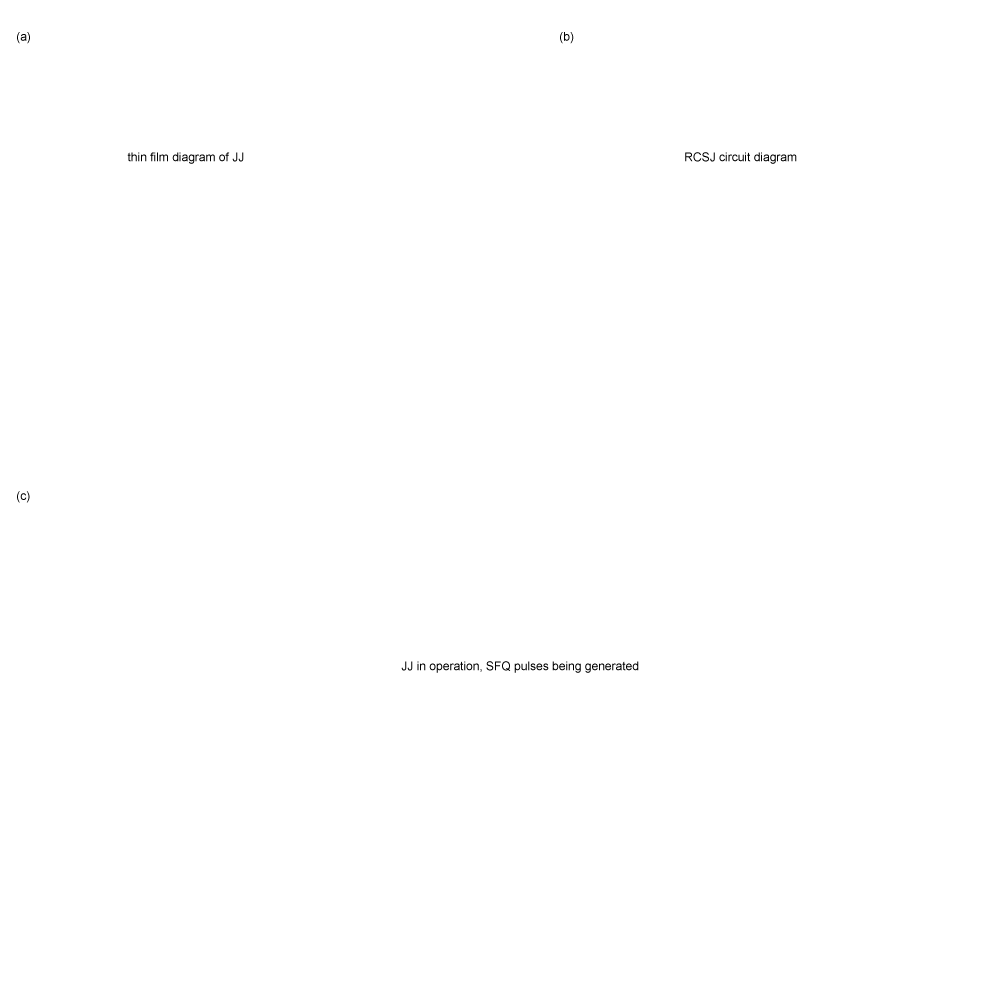
\includegraphics[width=8.6cm]{figures/jj.png}}
	\captionof{figure}{\label{fig:jj}Caption for JJ.}
\end{figure}
A JJ is created when two superconducting wires are separated by a thin tunneling barrier, as shown in Fig.\,\ref{fig:jj}(a). Excellent resources exist that describe the beautiful physics of JJs pedagogically \cite{ti1996,vatu1998,ka1999}, and it is our intention here to describe only very basic aspects of JJ operation relevant to the computing technology under discussion. 

When realized in hardware, any Josephson junction has some shunting capacitance and resistance, leading to the effective circuit shown in Fig.\,\ref{fig:jj}(b), which is referred to as the resistively and capacitively shunted junction (RCSJ) model. While a JJ can, in general, be either voltage biased or current biased, for simplicity we restrict our attention to current-biased junctions as they are more relevant to the operations at hand. One can see that in this model of the junction, there are three conduction paths in parallel. Perhaps the most important aspect of a JJ when used as a classical information-processing element is the fact that the junction has a critical current. This means the central, superconducting path can carry a current $I\le I_{\mathrm{c}}$ with exactly zero resistance and therefore zero voltage acorss the junction. However, if the current bias exceeds $I_{\mathrm{c}}$, the fraction $\Delta I = I-I_{\mathrm{c}}$ cannot be carried through the superconducting channel, and instead must be carried through the parallel conduction pathways, with DC components being shunted through the resistor. Under a bias exceeding $I_{\mathrm{c}}$, a voltage develops across the junction, and in general, this voltage will vary with time, even if the bias is constant, as we will describe in more detail shortly. 

One of the reasons JJs are so fascinating is that depending on the choice of circuit parameters, JJs can demonstrate many behaviors. Because a JJ has an intrinsic inductance, the circuit effective JJ circuit of Fig.\,\ref{fig:jj}(b) can operate as an $L-R-C$ oscillator circuit, leading to ringing behavior. Alternatively, with other parameter choices, the junction can demonstrate latching behavior, wherein a junction biased above its critical current will enter the resistive state and stay there until the current bias is dropped well below the critical current, thus exhibiting hysteresis. For the information processing applications under consideration, it is more advantageous to operate near critical damping.

Let us now consider the operation of a simple circuit employing a single JJ...

Need to touch on speed, flux quantization (need to introduce SFQ terminology, fluxon), JTL, flux storage, energy, $\Phi_0$, integral Vdt

\subsubsection{Superconducting digital logic}
Here we briefly review the history of using superconductors in digital computing. More detail can be found in Ref.\,\cite{li2012}. The origin of superconducting computing is nearly concurrent with the origin of the rest of digital computing. In that post WWII context, the first components developed were switches for digital systems. The goal was to implement a von Neumann architecture, the same pursuit as vacuum tubes and transistors. In was in this setting that Buck developed a switch wherein a superconducting wire with high critical field is wrapped around a superconducting wire with lower critical field. A current passing through the coil wire could be used to break superconductivity in the core wire. Such an element could be used for switching and current amplification. Dudley Buck referred to this device as a cryotron.

The cryotron was a strong candidate as a switch for binary computing when compared to vacuum tubes, but with the development of integrated circuits this bulk component was not competitive for scaling. Yet in the late 1960s and early 1970s, IBM developed an integrated circuit element based on JJs that behaved like Buck's cryotron \cite{an1980}. At that time, the materials for implementing superconducting integrated circuits were immature, and the device concepts for information processing were also under development. IBM chose to use Pb alloys as the material platform, and they chose to implement a latching logic \cite{lise1991}. This material platform was problematic, and nearly all contemporary efforts in superconducting logic utilize Nb as the predominant material for wiring and JJs (superconducting qubits are primarily based on Al). The latching logic IBM employed used the voltage across a JJ to represent information. As described above, a current-biased JJ can develop a voltage if the current bias exceeds $I\le I_{\mathrm{c}}$, and with a certain choice of the RCSJ circuit parameters, that junction can remain latched in the voltage state even after the current bias drops below $I\le I_{\mathrm{c}}$. Both the choice of Pb as a material platform and the choice to employ voltage-state logic ended up being problematic for IBM, and by the early 1980s IBM ceased its effort in superconducting digital logic.

The effort at IBM began before silicon microelectronic technology had far surpassed other approaches to digital logic, Moore's law had only recently been formulated \cite{mo1965}, and it certainly was not obvious which hardware would dominate for electronic computing. One of the motivations to use superconducting circuits was that they were simpler to fabricate than semiconducting circuits. Additionally, due to the intrinsic dynamics of JJs, they could be made to operate at extremely high speed with low energy per operation. Materials improvements led to the development of JJs based on Nb with AlO$_{x}$ as a tunneling barrier, and several efforts continued to explore JJ-based circuits for computing. In particular, the work by Likharev and others in the late 1980s and early 1990s developed a new type of logic for digital computing (see Refs.\,\cite{lise1991} and \cite{buli2001} for technical details and Ref.\,\cite{li2012} for a retrospective). Within this framework, the state of flux within a superconducting loop represents information: an empty loop represents a binary zero; a loop with one fluxon represents a binary one. This form of logic is referred to as flux-state logic, and it overcomes many of the weaknesses of voltage-state logic. Likharev and colleagues referred to this approach as rapid single-flux-quantum logic, and developed a family of gates to implement digital computing. Within this framework, a clock is distributed across all gates in the system, and logical operations proceed based on whether or not flux is present in certain loops during each clock cycle. 

The foundational work on flux-state logic \cite{lise1991,buli2001,li2012} occurred during the prime years of silicon microelectronic scaling. For this reason, it was difficult to foster a large effort in a competing technology, leading Likharev to later lament the oppressive impact incurred on other technologies as ``CMOS continued its victorious march.'' \cite{}. Yet interest in superconducting electronics for computing has continued, particularly in Japan, and as the scaling of silicon transistor technology has reached new barriers, attention has returned. In the US, the resurgence led to the IARPA Cryogenic Computing Complexity program, started in 2014, to develop high-performance superconducting digital computers. This effort, however, has not quickly led to circuits outperforming CMOS for digital computing. There are four reasons for this. We list them in order of severity. The first reason is that it is difficult to implement large arrays of compact memory cells with superconducting electronics \cite{}. This is very problematic when implementing the von Neumann architecture, as these digital efforts have aspired to do. The secondary reason is that distribution of a high-speed clock across many logic gates encounters obstacles, and the timing jitter of the gates leads to errors if the clock is too fast, largely eliminating speed advantages relative to CMOS. The third reason is that a superconducting system resides inside a cryostat. A high-performance computer will need extensive I/O, and this cannot be achieved straightforwardly with co-axial cables due to the high heat load such cables transfer from room temperature the the 4.2\,K stage where computation is performed. Optical approaches are being developed to overcome this challenge \cite{}, but optical sources or modulators often require on the order of a volt to encode a bit, while the SFQ pulses produced by JJs are on the order of a millivolt. This introduces the fourth problem limiting the success of superconducting electronics for digital computing: it is difficult for a superconducting circuit to change the state of a CMOS circuit. That is to say, it is difficult for a superconducting circuit to achieve sufficient voltage to switch the gate of a silicon transistor. Even if one intends to develop superconducting electronics to outperform silicon electronics specifically in the domain of digital logic, it is helpful (and perhaps vital) that the superconducting system be able to interface bi-directionally with semiconductors so the superconducting system can leverage the tremendous infrastructure of semiconductor integrated circuits. 

\vspace{3em}
still need in this section:
\begin{itemize}
\item description of RQL
\item description of AQFP, extreme energy efficiency, Landauer limit
\end{itemize}

\vspace{3em}
recent work on basic science of MJJs: cama2018,kamu2018,bakl2018
search bib for MJJ

\vspace{3em} 
discussion of superconducting electronics for sensing/particle detection

\vspace{3em}
Superconducting circuits can perform Boolean logic well enough to control networks of loop neurons and possibly qubits, but superconducting electronics are not poised to displace CMOS electronics for logic, particularly not in lightweight applications such as IoT and edge computing that have become so influential to the development of hardware for AI.

\subsubsection{Neurons based on Josephson junctions}
The development of superconducting digital electronics in the 1980s and 1990s was concurrent with the second wave of excitement regarding neural networks. Thus, several research groups developed circuits based on JJs to behave as neurons in ANNs, primarily in Japan. Following two conference proceedings in 1989 \cite{ai1989,og1989}, the first articles regarding JJ circuits for ANNs were published in 1991 \cite{hago1991,hiak1991}. The objective of the circuits was to perform the weighted summation and thresholding operations required in the computational primitives of ANNs. The circuits employed were similar to those utilized in superconducting digital logic, as were the basic concepts, such as using an up-down counter to implement synaptic weights \cite{hiak1991}. From the beginning, attention was paid to sculpting a sigmoidal transfer function to implement back-propagation as well as alternative circuits for achieving Hebbian-type learning \cite{hago1991}. The intrinsic threshold of a JJ upon being driven above its critical current was naturally used for thresholding \cite{hago1991}, and mutual inductors were identified as promising for addition of synaptic signals and fan-in \cite{hiak1991}. Little analysis was dedicated to anticipating scaling of such systems, although Ref.\,\onlinecite{hiak1991} claimed that achievable fan-out would be ``sufficiently large to implement large scale neural networks,'' and that ``fan-in is essentially unlimited.'' While the first assertion depends on one's definition of ``large scale'', subsequent analysis indicates that fan-out is a serious fundamental challenge for superconducting electronics, and fan-in reaches practical limitations due to the properties of mutual inductors, as we will discuss in more detail below.

Subsequent designs and experimental demonstrations were presented by Mizugaki et al. in 1994 \cite{mina1994a,mina1994b} and 1995 \cite{mina1995}. These circuits employed SQUIDs in various configurations for synaptic and neuronal responses. Again, digital concepts were employed, such as establishing the bit depth of possible synaptic weight values by adding additional DC SQUIDs. The focus remained on achieving feed-forward ANNs. Regarding fan-out, the intention was to use direct connections via superconducting wires to communicate between neurons. As stated in Ref.\,\onlinecite{mina1994a}, ``If it is necessary for a neuron circuit to drive a lot of another neurons, we can use biased JTLs...though the use of JTLs might reduce the integration scale.'' 

In 1997 Rippert and Lomatch at Northwestern University proposed neural circuits using similar principles of SFQ pulse generation rate representing activation, but new innovations were introduced regarding learning \cite{rilo1997}. The emphasis was still on ANNs rather than spiking neurons, and digital circuits were employed wherein higher-bit-depth synapses were achieved by adding junctions. This work began to explore Hebbian learning based on the temporal coincidence between two fluxons incident upon a JJ. In their circuit design, the coincidence window is determined by the temporal width of fluxons as well as the JJ bias current, and could achieve values of 1\,ps to 5\,ps. Reference \onlinecite{rilo1997} was the first to introduce a mechanism for metaplasticity in superconducting synapses wherein synaptic efficacy is updated through a Hebbian process, and the rate of Hebbian update is modified by additional circuits that adapt the Hebbian circuits. This work was before the term ``metaplasticity'' had become common in the neuroscience literature, but after the 1982 introduction of the BCM learning rule \cite{bico1982} that some consider the first example in computational neuroscience of a metaplastic synaptic mechanism \cite{cube2012}.

Efforts in superconducting neural circuits continued in Japan through the 2000s and 2010s \cite{koko2005,onko2009,hias2006,hias2007,onma2011,yaum2013}. The emphasis remained on ANNs implemented with circuits originally designed for digital logic. References \onlinecite{koko2005} and \onlinecite{onko2009} continued to explore and demonstrate the approach with up/down counters to represent a membrane potential with the output rate of fluxons representing the neuron's activation. Networks of these circuits were simulated solving a combinatorial optimization problem in Ref.\,\onlinecite{onma2011}, and more attention was paid to generating an accurate sigmoid function for back-propagation in Ref.\,\onlinecite{yaum2013}. In 2013 in Italy, a small network of SQUID-based neurons was demonstrated and used to implement an XOR gate when trained through examples using an genetic algorithm in Ref.\,\onlinecite{chca2013} .

Throughout Refs.\,\onlinecite{hago1991,hiak1991,mina1994a,mina1994b,mina1995,rilo1997,koko2005,onko2009,onma2011,yaum2013}, a neuron's activation was represented by the rate of production of fluxons, which becomes the time-averaged output current after low-pass filtering. By contrast, Refs.\,\onlinecite{hias2006} and \onlinecite{hias2007} proposed designs for leaky integrate-and-fire neurons that sum fluxons and produce a single flux quantum upon reaching threshold, much more in the spirit of single-flux-quantum digital electronics. To my knowledge, this was the first proposal to use superconducting circuits for spiking neurons. Input fluxons were stored in superconducting loops, and the number of input fluxons required to reach threshold was set in hardware by the number of JJ storage loops in the integrator. The leak rate was established by adding a resistance to one of the loop, giving exponential current decay with an $L/r$ time constant. Fan-out was envisioned to occur through JTLs and splitters, while fan-in was envisioned to utilize confluence buffers. No scaling analysis regarding the possible number of connections was presented.

In 2010, Crotty, Schult and Segall at Colgate University proposed a different approach to integrate-and-fire neurons \cite{crsc2010}. Rather than focusing on achieving weighted summation and nonlinear activation for ANNs, this work was oriented toward using JJ circuits to model neurons and their dynamics. Toward this end, they also adapted a circuit from superconducting digital electronics. The neuron circuit proposed in Ref.\,\onlinecite{crsc2010} is based on the DC-to-SFQ converter. Segall and his colleagues identified a correspondence between the behavior of each of the two junctions in the circuit and ionic currents across a neuron's cell membrane, with one junction behaving like a Na$^+$ current producing the rise of an action potential, and another junction behaving like a K$^+$ current quenching the action potential and restoring the membrane potential to its resting level. It was estimated that a cortical column with $10^4$ neurons could be simulated with JJ circuits on a single chip, but an interconnection scheme was not proposed. Subsequent work from the Colgate group simulated \cite{segu2014} and experimentally realized \cite{sele2017} synchronization dynamics of a two coupled neurons. In these neurons, a pulse consisting of a single flux quantum represents an action potential, and an RC circuit achieves synaptic leak, resulting in neuronal firing up to 25\,GHz with $10^{-17}$\,J/spike. 

While 10\,aJ per action potential is low, some aspire to far lower operation. As mentioned in Sec.\,\ref{sec:superconductors}, there are multiple ways to use JJ circuits to implement digital logic. Correspondingly, there are multiple ways to use similar circuits to implement neural functions. While much of the work on superconducting neurons utilizes circuits most similar to SFQ logic circuits, an emerging branch utilizes AQFP circuits (see Sec.\,\ref{sec:superconductors}). The energy efficiency of AQFP circuits derives from the fact that the junctions involved are never driven above their critical current, and so never produce fluxons. Instead, the Josephson nonlinear inductance is employed to establish nonlinear current input/output relations. Utilization of adiabatic cells for ANNs was first introduced in 2016 by Schegolev et al. in Russia \cite{sckl2016}, and the ideas have been further developed in Refs.\,\onlinecite{klsc2018} and \onlinecite{sosc2018}, where the authors proposed to utilize MJJs for synapses in conjunction with adiabatic neurons.  Work from Katayama et al. in Japan \cite{kafu2018} has developed related concepts flux-biased SQUIDs to achieve a sigmoidal transfer function suitable for back-propagation for training ANNs.

As mentioned in Sec.\,\ref{sec:superconductors}, Josephson junctions with a ferromagnetic material in the tunneling barrier can be used as a memory element in superconducting circuits \cite{vevi2013}. The state of magnetic order can be used to tune the critical current across a broad range, and this can be used to steer a bias current. The use of MJJs as a synapse in superconducting neural circuits was first proposed in 2016 by Russek et al. \cite{ru2016} and has been subsequently demonstrated by Schneider et al. \cite{scdo2018} in 2018. Further theoretical analysis of the use of MJJs for establishing synaptic weights in ANNs based on similar SQUID neurons to those discussed above \cite{hiak1991} was presented Ref.\,\cite{scdo2018b}, wherein simulation of nine-pixel image classification was shown with 3\,ns inference time per image. 

While all superconducting electronic neural systems mentioned in the section have utilized circuits based on JJ and their associated nonlinearities and thresholding behavior, neuron circuits based on quantum phase-slip junctions (QPSJs) have also recently been proposed \cite{chgo2018}. QPSJs are the dual to JJs, and thus corresponding dual circuits can be conceived to perform neural functions. QPSJs also have thresholding behavior and may offer further advantages in energy efficiency. These devices are still being developed, and one technical challenge is that one-dimensional superconducting wave functions must be achieved, which requires lithography down to about 10\,nm, making initial demonstrations as well as future scaling potentially more difficult than with JJs.

\subsubsection{Strengths and weaknesses of JJ circuits for neural operation}
In Refs.\,\onlinecite{hago1991,hiak1991,mina1994a,mina1994b,mina1995,rilo1997,koko2005,onko2009,hias2006,hias2007,onma2011,yaum2013,crsc2010,segu2014,sele2017,sckl2016,klsc2018,sosc2018,ru2016,scdo2018,scdo2018b,chgo2018}, five arguments have been forth regarding why superconducting circuits might outperform semiconducting circuits for neural computing: 1) JJs are faster than transistors, so JJ neurons and synapses will be faster than their silicon counterparts; 2) JJs consume less energy per operation than transistors, so superconducting neural systems will be more energy efficient; 3) JJs are highly nonlinear and have native thresholding and spiking behavior, so synaptic and neuronal circuits based on JJs can be implemented simply with few JJs; 4) superconducting transmission lines are lossless, so communication in superconducting neural systems will be superior to semiconducting neural systems using normal metal interconnects; and 5) due to their low power density, superconducting devices can be stacked in three dimensions with multiple planes of JJs, whereas the difficulty of removing heat from transistors precludes multiple active layers in a CMOS process. While I am a proponent of using JJ circuits for synaptic and neuronal functions, these arguments do not all hold up to scrutiny. As a broad comment, nowhere in Refs.\,\onlinecite{hago1991,hiak1991,mina1994a,mina1994b,mina1995,rilo1997,koko2005,onko2009,hias2006,hias2007,onma2011,yaum2013,crsc2010,segu2014,sele2017,sckl2016,klsc2018,sosc2018,ru2016,scdo2018,scdo2018b,chgo2018}, is a system-level analysis of a large network presented. Neural systems are complex with many device and circuit interdependencies across various scales of the network. To analyze claims about full systems based on the performance of a device in an isolated context can be misleading. To further illustrate these issues, let us consider each of the above arguments.

\vspace{1em}
\textit{1) JJs are faster than transistors, so JJ neurons and synapses will be faster than their silicon counterparts.} \newline It is true that the intrinsic time constants of JJ are shorter than transistors. Yet the cutoff frequency of a transistor does not limit the speed of CMOS neural networks directly. Because CMOS neural networks have reached a sufficient stage of maturity, full, functional systems can be analyzed. We find that at the scale of 100,000 neurons, event rates are limited to 1\,kHz per neuron \cite{payu2017}, and by 100 million neurons it is limited to 10\,Hz \cite{kuwa2017}, and this poor scaling results from the communication infrastructure, not the elemental device speed. It may be possible that large networks of JJ neurons are faster than large networks of transistor neurons, but we cannot conclude this until we know how communication will occur in these networks.

\vspace{1em}
\textit{2) JJs consume less energy per operation than transistors, so superconducting neural systems will be more energy efficient.} \newline At the device level, this argument seems well-founded, especially if adiabatic principles of operation are employed. Yet again we must think at the system level. The power required to operate a system at 4\,K in a background at 300\,K can be modeled as
\begin{equation}
\label{eq:power_to_operate_cryo}
P_{\mathrm{tot}} = m P_{\mathrm{dev}} + P_{\mathrm{0}},
\end{equation}
where $P_{\mathrm{dev}}$ is the power dissipated by the devices comprising the system due to normal operation, and $P_{\mathrm{0}}$ is the power required simply to cool the devices below to the operating point, which is 4\,K for most superconducting systems under consideration for this form of computation. This power is at least 100\,W for contemporary cryogenic systems, and is often 1\,kW, even when there are zero neurons in the system. The slope $m$ represents watts of cooling power required to stay below 4\,K per watt of device power dissipated due to operation. The theoretical limit is given by the Carnot efficiency, and when cooling from 300\,K to 4\,K this number is 150 watts per watt. In practice, it is often approximated as 1000 watts per watt. Thus, if we plan to operate the artificial neural system on earth, we should budget 1\,kW of power just to turn it on, and we should budget an additional 1\,kW of system power for each watt dissipated by the devices. This clearly limits the application spaces where superconducting systems are candidates to outperform semiconducting systems with regard to power consumption. Much of modern AI hardware aspires to play a role in small, deployable devices. Superconductors will never be useful in cell phones, the internet of things, or edge computing. Systems based on JJs may be more efficient than systems based on transistors, but this will only become relevant for systems large enough that the term $P_{\mathrm{0}}$ is tolerable. The domain of superconductors in neuromorphic supercomputing. High-$T_{\mathrm{c}}$ materials are unlikely to change this situation because the materials involved make fabrication of dense, integrated circuits very difficult, and operating of JJs at higher temperature is very noisy, even if the underlying material has a high $T_{\mathrm{c}}$ \cite{lise1991} (check this ref). 
  
  \vspace{1em}
\textit{3) JJs are highly nonlinear and have native thresholding and spiking behavior, so synaptic and neuronal circuits based on JJs can be implemented simply with few JJs.} \newline To me, this is the most compelling argument in favor of superconducting neural systems. Josephson junctions are ideal for performing the synaptic, dendritic, and neuronal behaviors we seek. This is most apparent when implementing spiking neurons that fully utilize the time domain. Most of the work to date in superconducting neural circuits has focused on generating nonlinear transfer functions, essentially for steady-state operation in feed-forward neural networks \cite{hago1991,hiak1991,mina1994a,mina1994b,mina1995,rilo1997,koko2005,onko2009,onma2011,yaum2013,sckl2016,klsc2018,sosc2018,ru2016,scdo2018,scdo2018b,chgo2018}, but we will argue in Sec.\,\ref{sec:superconductingOptoelectronic} that JJ circuits similar to the spiking neurons of Segall and co-workers \cite{crsc2010,segu2014,sele2017} can perform many desirable synaptic, dendritic, and neuronal functions going far beyond simple, point-neurons.

\vspace{1em}
\textit{4) Superconducting transmission lines are lossless, so communication in superconducting neural systems will be superior to semiconducting neural systems using normal metal interconnects.} \newline The dissipationless nature of superconducting wires is an extraordinary benefit to neural computing, digital logic, and quantum computing alike. But dissipationless transmission lines alone are not sufficient to enable an interconnection network, particularly when spiking is involved. The major problem with communication on metal wires is not resistance, but capacitance, as described in Sec.\,\ref{sec:electronics}. Likewise, superconducting interconnects must contend with problems related to inductance. If the output of a neuron is one or more fluxons generated by a JJ, the current associated with each fluxon will be $\Phi_0/L$, where $L$ is the total inductance of the output lines being fed by the JJ. As more connections are added, the inductance gets larger, the current gets smaller, and the neuron eventually cannot source enough current to directly feed all of its synaptic connections. One solution to this problem is to use JTLs and pulse splitters to provide gain as a pulse porpagates through and branches across the interconnection network. Other approaches to fan-out are discussed in Sec.\,\ref{sec:superconducting_interconnects}, but it is likely that an active interconnection network of JTLs and splitters will be required to achieve communication from one spiking neuron to many synaptic connections. Active transmission lines dissipate power, and so arguments related to the lossless nature of superconducting transmission lines are not applicable. Again, one must propose an interconnection network adequate at the system level to assess the full benefits of lossless communication lines. It is not clear that routing of fluxonic signals from JJ neurons across large networks can be achieved without resorting to address-event representation, as is done by CMOS. If AER proves necessary, superconducting circuits will have much more difficult road ahead than CMOS, because AER places severe demands on memory, and superconducting circuits struggle with dense memory.

For certain feed-forward superconducting ANNs, particularly those based on AQFP circuits, it is not necessary for a neuron to produce an output that switches a junction, and passive transmission lines with high inductance may suffice. In this case, the high inductance will lead to reduced speed when changing the inputs to the network, so the interconnection network must be analyzed in conjunction with the inference latency, and speed/scaling trade-offs will be present.

\vspace{1em}
\textit{5) Due to their low power density, superconducting devices can be stacked in three dimensions with multiple planes of JJs, whereas the difficulty of removing heat from transistors precludes multiple active layers in a CMOS process.} \newline This could be another tremendous advantage of superconducting circuits for long-term scaling. The power density of JJ circuits is low enough that many layers could be stacked while maintaining the ability to conduct heat to a bath of liquid helium, particularly when the circuits are participating in temporally sparse neural activity. However, in practice it is difficult to produce wafers with multiple planes of JJs \cite{to2016}, although there is plenty of room for development through future research. Three-dimensional integration of complex JJ neural circuits appears possible in principle, and it remains to be seen how far it can go in practice, but if successful could bring exceptional advantages for large-scale systems.

\vspace{1em}
In this section we reviewed 30 years of work on superconducting neural circuits, and we described their strengths as well as their weaknesses. 

\vspace{1em}
\begin{itemize}
\item mina1994a anticipated problems with superconducting lines, JTLs, and scaling
\item early works used digital concepts, adding active circuits to increase synaptic bit depths, hwereas we now plan to use purely passive Lr loops, enabled by high-kinetic-inductance materials
\item neuronal firing: mina1994a, mina1995, hagu1991 all use time-averaged output of SFQs from JJ as signal representing activation (not 1 fluxon action potential)
\item advantages of superconductors for 3D integration seen in hiak1991
\item temporal coincidence: compare/contrast with rilo1997 where use $\Delta t$ of JJ. also metaplasticity
\end{itemize}

\vspace{1em}
Design of a Power Efficient Artificial Neuron Using Superconducting Nanowires
\cite{tose2019}